While state-of-the-art research and practice have been well-established for deriving control-flow and program dependencies for entire programs, there have been little to no advancements in conducting such a program dependence analysis for partial programs. In this proposal, we set out to investigate and develop {\tool}, a {\em \underline{Neural} Network-Based \underline{P}rogram \underline{D}ependence \underline{A}nalysis} infrastructure, that enables (partial) program dependence analysis. Adopting such a neural network-based approach has the benefit of potentially speeding up dependency discovery when compared to traditional program analysis tools.

\begin{center}
    \begin{minipage}{33.5em}
    The key philosophy that drives our work is that {\em the dependence analysis of partial code can be learned from the dependence analysis for entire programs via the wealth of information obtained from ultra-large-scale, open-source software repositories}.
    \end{minipage}
\end{center}

We draw motivation for such a data-driven, learning-based approach from the following. First, ultra-large-scale software repositories, e.g., GitHub (7M+ projects) and SourceForge (700k+ projects), contain an enormous collection of programs. These repositories amount to 1B+ lines of code, 10M+ revision logs, and 3M+ issue reports. This wealth of knowledge is an excellent source for {\tool}. Hindle {\em et al.}~\cite{naturalness-icse12} have shown that code has high repetitiveness and predictability and can be captured well by statistical models. Thus, we expect to build ML/DL models to learn from those repositories. Second, in an empirical study on the repetitiveness, containment, and composability of PDGs in open-source projects, the PI group~\cite{msr16} reported that among 17.5M PDGs with 1.6B PDG subgraphs, 14.3\% of the PDGs have all of their subgraphs repeated across different projects. Furthermore, in 15.6\% of the PDGs, at least 90\% of their subgraphs are likely to have appeared before in other projects. Thus, {\tool} could learn from PDGs with complete program dependencies retrieved from existing code repositories and derive dependencies for the partial code fragment under study. Broadly, such a partial program dependence analysis infrastructure is similar in spirit to neural network-based dependency parsing approaches in natural language processing (NLP), which learn the dependencies signifying the semantic relationships between words in a sentence from the text corpora.

To accomplish this task, we propose the following thrusts of research:

\vspace{3pt}
\noindent \textbf{[Thrust 1] Benchmark Dataset Construction.} Traditional program analysis tools are noisy, i.e., prone to false positives, particularly for flow-based analyses. We plan to mitigate such issues by collecting high-quality source code repositories and extracting their CFG/PDGs across varying criticality levels (each representing a real-world scenario) by combining diverse program analysis tools. Benchmark datasets thus created can help facilitate a learning-based approach to partial program dependence analysis.

\vspace{3pt}
\noindent \textbf{[Thrust 2] Neural Network-Based Program Dependence Analysis Infrastructure.} The basic infrastructure for learning-based program dependence analysis has two main tasks. First, it learns the well-defined syntactic and semantic information in source code by leveraging the program representations obtained for complete programs in the benchmark datasets. Next, given either a complete or partial code fragment, the trained model infers the inter-statement program dependencies to realize the CFG/PDG for the fragment.

\begin{figure*}[ht]
\begin{center}
    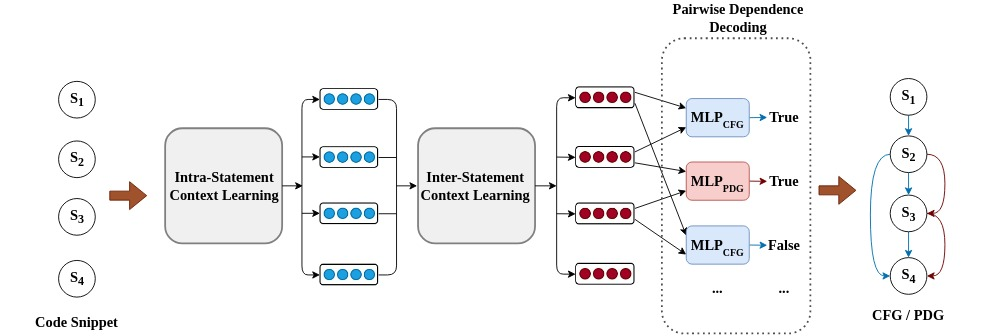
\includegraphics[width=\textwidth]{model-abstract.jpg}
    \caption{Preliminary Design for \tool Model Infrastructure.}
    \label{fig:model}
%    \vspace{-12pt}
\end{center}
\end{figure*}

\vspace{3pt}
\noindent \textbf{[Thrust 3] Enabling Fragment-Level Vulnerability Detection with \tool.} Vulnerability detection in code fragments can be facilitated as follows: (a) employing \tool infrastructure to predict the CFG/PDG for a given code fragment; (b) leveraging an existing automated VD tool that utilizes the predicted CFG/PDGs to identify the presence of vulnerabilities in partial code fragments.
